%! Author = lili
%! Date = 8/13/26

\section{Abgabe 2.3}\label{sec:abgabe-2.3}

\subsection{HA 2.3.1 \abhaken}\label{subsec:ha-2.3.1}
Der Glashersteller Crystal Clear produziert unter anderem Rotweingläser. Im Schnitt weist eins von tausend produzierten Rotweingläsern kleine Bläschen auf. Diese Gläser werden als B-Ware deklariert.

\begin{auf}[(a) Geben Sie einen geeigneten Wahrscheinlichkeitsraum an, der es erlaubt, die folgenden Aufgabenteile zu bearbeiten. Diskutieren Sie, welche Annahmen Sie machen müssen, um Ihre Wahl des Wahrscheinlichkeitsraums zu rechtfertigen.]
    $\ $
    \begin{figure}[H]
        \centering
        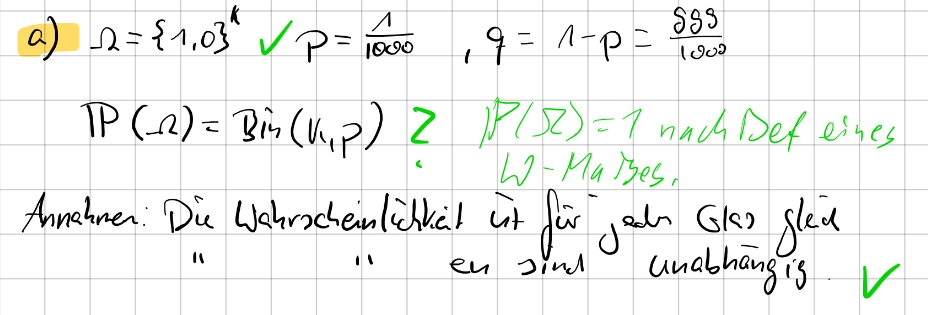
\includegraphics[width=0.8\linewidth]{images/lösungen/wts231a}
    \end{figure}
\end{auf}

(b) Berechnen Sie für jedes $k\in\{500,1000,2000\}$ die Wahrscheinlichkeit, dass sich unter $k$ produzierten Rotweingläsern mindestens ein Weinglas befindet, das kleine Bläschen aufweist.
\begin{auf}[(i) Führen Sie die Rechnung sowohl mit Hilfe der Poisson-Approximation...]
    $\ $
    \begin{figure}[H]
        \centering
        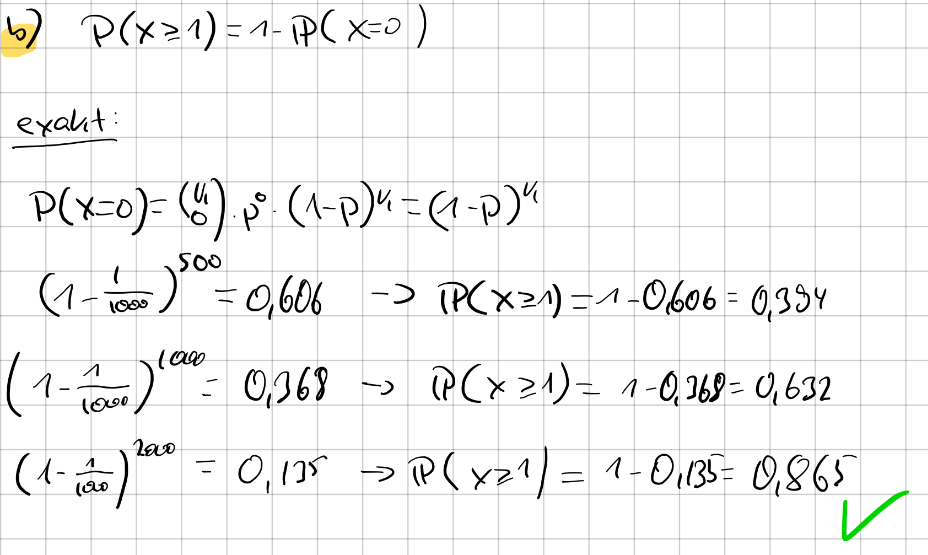
\includegraphics[width=0.8\linewidth]{images/lösungen/wts231bi}
    \end{figure}
\end{auf}

\begin{auf}[(ii) ... als auch mit Hilfe der Normal-Approximation durch. Berechnen Sie zum Vergleich auch das exakte Ergebnis.]
    $\ $
    \begin{figure}[H]
        \centering
        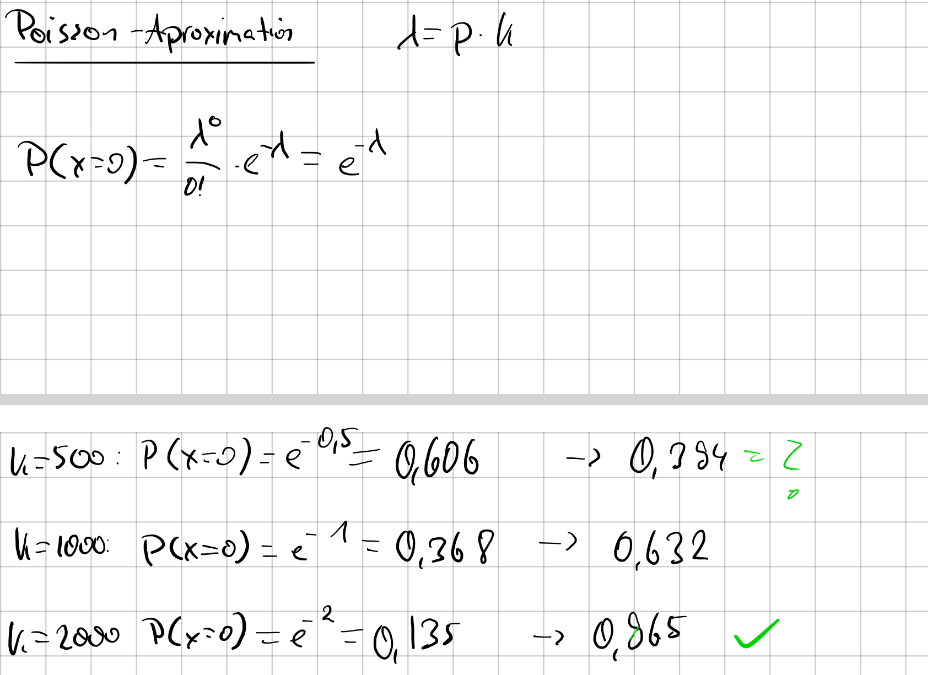
\includegraphics[width=0.8\linewidth]{images/lösungen/wts231bii}
    \end{figure}
\end{auf}

\begin{auf}[(c) Welche der Approximationen ist besser? Warum?]
    Die Poisson-Approximation ist deutlich näher an der exakten Lösung als die Normalapproximation.
    Dies liegt daran, dass die Poisson-Approximation für große n (in dem Fall der Aufgabe k), kleine
    p und kleine k (hier 0) besonders genau ist.
\end{auf}

\subsection{HA 2.3.2 \abhaken}\label{subsec:ha-2.3.2}

\begin{auf}[(a)]
    $\ $ \\
    \paragraph{z.z.:} $\pe(Z \geq \wfk - x) = \Phi \left( \frac{x}{\sigma} \right) \quad \forall x \in \rz$ \\
    \paragraph{Beweis:} $\pe(Z \geq \wfk - x) = \pe(Z - \wfk \geq  - x) = \pe\left( \frac{Z - \wfk}{\sigma} \geq  \frac{- x}{\sigma} \right)$ \\
    Dann $Z$ mit $Y = \frac{Z - \wfk}{\sigma}$ standardisieren, so folgt:
    $\pe\left( Y \geq  \frac{- x}{\sigma} \right) = 1 - \Phi\left(  \frac{- x}{\sigma} \right) \Leftrightarrow  1 - \Phi\left(  \frac{- x}{\sigma} \right)  = \Phi \left(  \frac{x}{\sigma}  \right) $
\end{auf}

\begin{auf}[(b)]
    $\ $
    \begin{figure}[H]
        \centering
        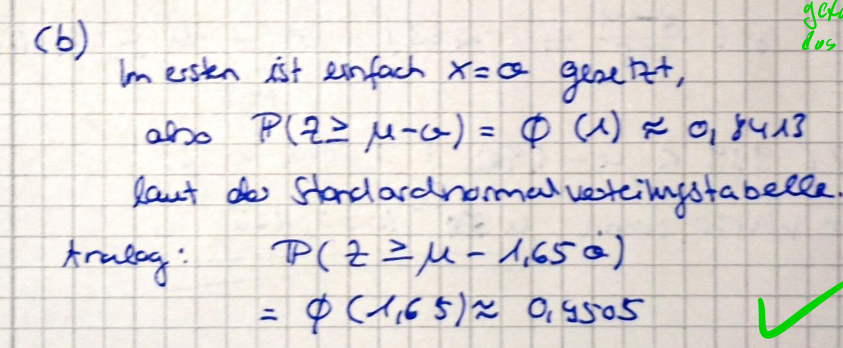
\includegraphics[width=0.8\linewidth]{images/lösungen/wts232b}
    \end{figure}
\end{auf}


\begin{auf}[(c)]
    $\ $
    \begin{figure}[H]
        \centering
        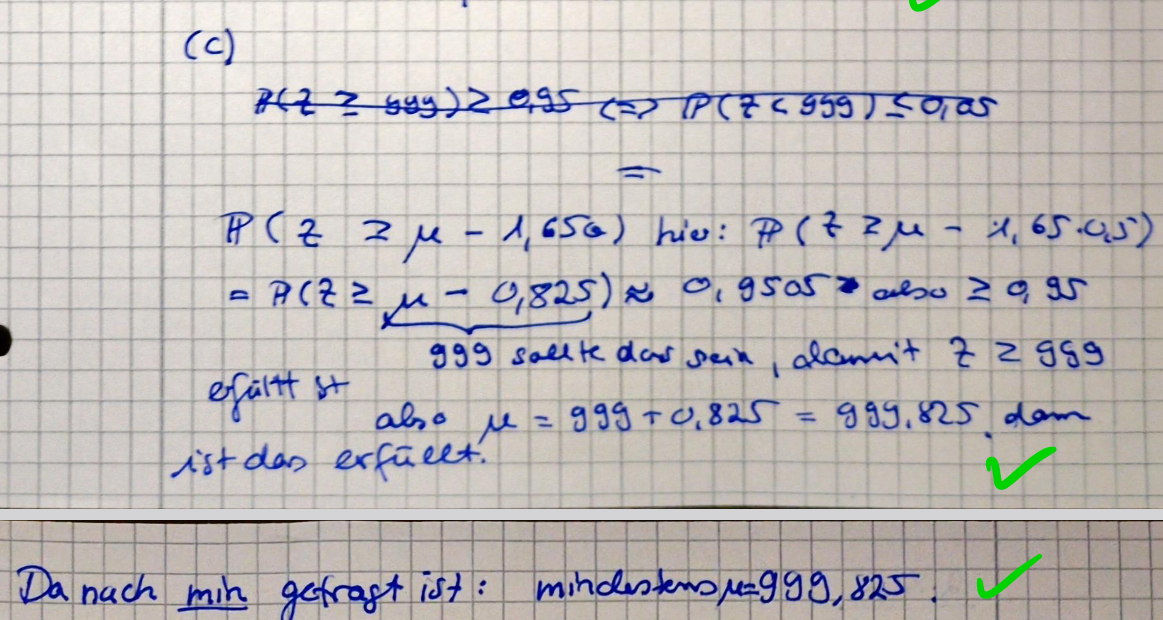
\includegraphics[width=0.8\linewidth]{images/lösungen/wts232c}
    \end{figure}
\end{auf}



\begin{auf}[(d)]
    $\ $
    \begin{figure}[H]
        \centering
        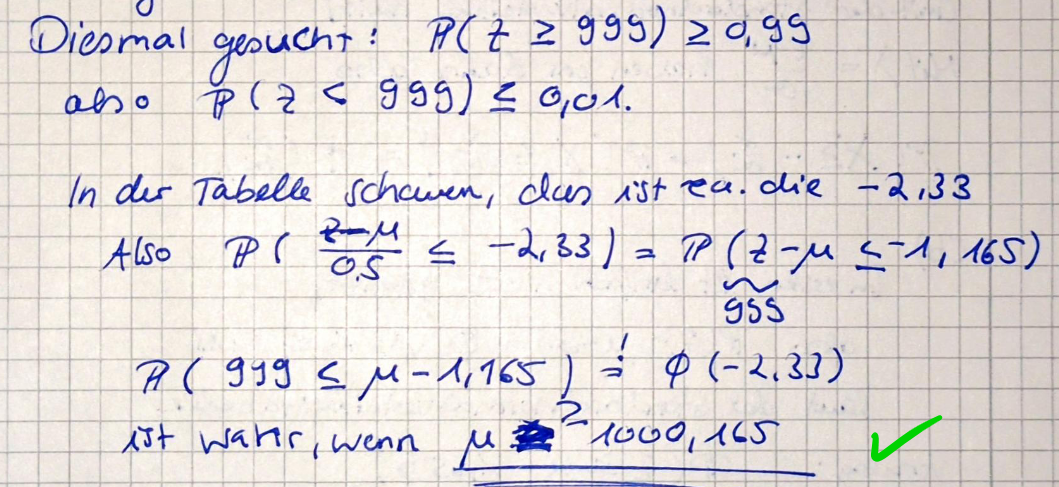
\includegraphics[width=0.8\linewidth]{images/lösungen/wts232d}
    \end{figure}
\end{auf}


\subsection{HA 2.3.3}\label{subsec:ha-2.3.3}